\section{Introduction}
The physics background for this note is essentially the same as in Belle notes $\#805$, $\#878$, $\#902$ and $\#1347$~\cite{BelleNote1,BelleNote2,BelleNote3,BelleNote4} which describe the measurement of the Collins effect for charged pions and kaons. 
In Semi-inclusive Deep Inelastic Scattering~(SIDIS) and polarized $p+p$ collisions, the Collins effect can be used to access the transversity distribution function $h_1(x)$. Together with $f_1$, the unpolarized parton distribution function (pdf), and $g_1$, the helicity distribution function,  transversity is needed to describe the spin structure of the nucleon at leading twist and in a collinear picture. Unlike $f_1$ and $g_1$ , $h_1$ cannot be accessed in inclusive measurements. It is a chiral odd function and is highly suppressed in inclusive deep inelastic scattering experiments. In SIDIS or $p+p$ collision experiments, the transversity distribution function couples with the Collins Fragmentation function which serves as a quark polarimeter. The Collins FF has to be measured separately, and the cleanest way to do this is $e^+e^-$ annihilation where a $q\bar{q}$ pair is created and then fragments into hadrons. Measurement of Collins fragmentation function provides information to extract the transversity distribution function from SIDIS processes. Collins fragmentation functions have been measured for kaons and charged pions by $BABAR$ and Belle. In this thesis, for the first time the Collins analysis for $\pi^{0}$ and $\eta$ will be presented. 
%\include{chapters/chapter1}

\subsection{Physics}
\subsubsection{SIDIS Cross subsection}
\label{sec:SIDIScrosssubsection}
\begin{figure}[ht]
  \centering
  \includegraphics[width=0.8\textwidth,natwidth=610,natheight=642]{figure_theory/SIDIS.eps}
  \caption{Semi-inclusive deep-inelastic scattering process~(SIDIS)}
  \label{fig:SIDIS}
\end{figure}

Consider the semi-inclusive deep-inelastic scattering process $\ell+N \rightarrow \ell'+h+X$ (Fig.~\ref{fig:SIDIS}). The lepton $\ell$ with momentum $l$ scatters off a nucleon $N$ with momentum $P$ where the outgoing hadron $h$ and lepton $\ell'$ are detected while the debris $X$ remains unknown. Let $P_h$ and $l'$ be the momentum of the outgoing hadron and lepton, respectively. The invariants $x,y,z$ can be defined by $x \equiv Q^2/2P \cdot q$, $y \equiv \nicefrac{P\cdot q}{P \cdot l}$ and $z_h \equiv \nicefrac{P\cdot p_h}{P \cdot q}$. The cross subsection for SIDIS can be written in terms of the leptonic and the hadronic tensor as in Eq.~\ref{eqn:SIDIScrosssubsection}. In the calculation the Born approximation is used, namely, the scattering reaction takes place by single photon exchange. This subsection is based on Ref.~\cite{Boer:2003cm, AsyInPolarizedHadronProductionInEE,AsymmetryInEE,CompleteTreeLevel,TransversePN}.

Here $L_{\mu\nu}$ is the leptonic tensor and $2M\mathcal{W}^{\mu\nu}$ is the hadronic tensor.~\cite{TransversePN,CompleteTreeLevel}
\begin{equation}
\frac{d\sigma}{dx_Bdydz_hd^2\boldsymbol{q}_T} = \frac{\pi \alpha^2}{2Q^4}yz_hL_{\mu\nu}2M\mathcal{W}^{\mu\nu}
\label{eqn:SIDIScrosssubsection}
\end{equation}
The leptonic tensor can be calculated by Eq.~\ref{eqn:leptontensor}, where $u_l$ is the in-going lepton's four-component spinor:
\begin{equation}
\begin{aligned}
L_{\mu\nu}  =\sum_{s_{l'}}[\bar{u}_{l'}(\ell',s_{l'})\gamma_{\mu}u_l(\ell,s_l)]^{\ast}[\bar{u}_{l'}(\ell',s_{l'})\gamma_{\nu}u_l(\ell,s_l)] \\
=Tr[(\slashed{\ell}+m_l)\frac{1}{2}(1+\gamma_5\slashed{s}_l)\gamma_{\mu}(\slashed{\ell}'+m_l)\gamma_{nu}],
\end{aligned}
\label{eqn:leptontensor}
\end{equation}
and neglecting the lepton masses
\begin{equation}
L_{\mu\nu}  =\delta_{\lambda\lambda'}(2l_{\mu}l'_{\nu}+2l_{\nu}l'_{\nu}-Q^2g_{\mu\nu}+2i\lambda\epsilon_{\mu\nu\rho\sigma}q^{\rho}l^{\sigma}).
\label{eqn:leptontensor2}
\end{equation}
In terms of the parton's transition current $J^{\mu}$, the hadronic tensor is given by~\cite{CompleteTreeLevel}:
\begin{equation}
\begin{aligned}
2M\mathcal{W}_{\mu\nu}\sim \frac{1}{(2\pi)^4}\sum_X\int\frac{d^3P_X}{(2\pi)^32P_X^0}(2\pi)^4\delta^4(q+P-P_X-P_h) \\
\times \langle PS|J_\mu(0)|P_X;P_hS_h\rangle\langle P_X;P_hS_h|J_\nu(0)|PS\rangle\\
%2M\mathcal{W}_{\mu\nu}= \frac{1}{(2\pi)^4}\sum_ae^2_a\sum_X\int\frac{d^3P_X}{(2\pi)^32E_X}\int\frac{d^4k}{(2\pi)^4}\int\frac{d^4\kappa}{(2\pi)^4} \\
= \frac{1}{(2\pi)^4}\sum_ae^2_a\sum_X\int\frac{d^3P_X}{(2\pi)^32E_X}\int\frac{d^4k}{(2\pi)^4}\int\frac{d^4\kappa}{(2\pi)^4} \\
\times (2\pi)^4\delta^4(P-P_X-k)(2\pi)^4\delta^4(k+q-\kappa)(2\pi)^4\delta^4(\kappa-P_h-P_X) \\
\times [\bar{\Xi}(\kappa;P_h,S_h)\gamma^\mu\Phi(\kappa;P,S)]^\ast[\bar{\Xi}(\kappa;P_h,S_h)\gamma^\mu\Phi(\kappa;P,S)],
\label{eqn:hadronictensor}
\end{aligned}
\end{equation}
with $S$,$P$ the spin and momentum of the nucleon, and $S_h$,$P_h$ the spin and momentum of the detected hadron, respectively. $k$ and $\kappa$ stand for the quark momenta before and after scattering. Fig. \ref{fig:SIDISbulb} depicts the momenta of the quark and hadron, the quark-quark correlation matrix inside the nucleon $\Phi$ and the quark-quark correlation matrix $\Xi$ in the fragmenting process.~\cite{TransversePN}  %The subscript $a$ is a mark for quark flavor. 

\begin{figure}[ht]
  \centering
  \includegraphics[width=0.8\textwidth,natwidth=610,natheight=642]{figure_theory/SIDIS_Feynman.eps}
  \caption{SIDIS handbag diagram}
  \label{fig:SIDISbulb}
\end{figure}
In the parton model, a parton is viewed as a quasi-free particle and described by a transition current $J^{\mu}$. The virtual photon strikes a parton, quark or antiquark, and this parton fragments into the final state hadron. Eq.~\eqref{eqn:hadronictensor} uses the parton model assumption that a quasi free quark fragments after scattering, and the quark current $\bar{\Xi}(\kappa;P_h,S_h)\gamma^\mu\Phi(\kappa;P,S)$ can be divided into two soft parts, $\Phi$ and $\Xi$ (cf.~Eqs.~\ref{eqn:phi}~\ref{eqn:xi},respectively), and treated independently. 

Fig.~\ref{fig:SIDISbulb} is the handbag diagram of the SIDIS process. The lower blob represents the quark-quark correlation inside the nucleon while the upper blob characterizes the fragmentation process. As only leading twist contributions are taken into account, there is no gluon radiation present in this Feynman diagram. 
  
\begin{equation}
  \begin{split}\Phi_{i,j}(k;P,S)=\sum_X\int\frac{d^3\boldsymbol{P}_X}{(2\pi)^32E_X}(2\pi)^4\delta^4(P_X+k-P)\phi_i(k;P,S)\\ \times \bar{\phi}_j(k;P,S)
=\int d^4\xi e^{ik\cdot\xi}\langle PS|\bar{\psi}_j(0)\psi_i(\xi)|PS\rangle
\label{eqn:phi}
  \end{split}
\end{equation}

\begin{equation}
\begin{split}
\Xi_{ij}(\kappa;P_h,S_h) %= \sum_X\int\frac{d^3\boldsymbol{P}_X}{(2\pi)^32E_X}(2\pi)^4\delta^4(P_h+P_X-\kappa)\times\chi_i(\kappa;P_h,S_h)\bar{\chi}_i(\kappa;P_h,S_h) \\
=  \sum_X\int\frac{d^3\boldsymbol{P}_X}{(2\pi)^32E_X}\int d^4\xi e^{i\kappa\cdot\xi}\times\langle 0|\psi_i(\xi)|P_hS_h,X\rangle \\
\times \langle P_hS_h,X|\bar{\psi}_j(0)|0\rangle
\label{eqn:xi}
\end{split}
\end{equation}
 The hadronic tensor can be expressed as the product of inside nucleon dynamics and the fragmentation process:
\begin{equation}
\mathcal{W}^{\mu\nu}  = \sum_ae_a^2\int\frac{d^4k}{(2\pi)^4}\delta^4(k+q-\kappa)Tr[\Phi\gamma^{\mu}\Upxi\gamma^{\nu}].
\label{eqn:hadronictensor3}
\end{equation}

\subsubsection{Quark Correlation Matrix} 
SIDIS is dominated by contributions from the light cone. The constructor projectors on the light cone are:
\begin{equation}
\begin{aligned}
\mathcal{P}_\pm=\frac{1}{2}\gamma^\mp\gamma^\pm.
\label{eqn:LC}
\end{aligned}
\end{equation}
In the $hN$ collinear frame, by neglecting terms that are suppressed by $\mathcal{P}^+$, the Sudakov decomposition for quark momenta and spin vector $S$ are:
\begin{equation}
\begin{aligned}
       k&=[\frac{(k^2+\boldsymbol{k}^2_T)}{2xP^+},\boldsymbol{k}_T] \approx xP+k_T, \\
       \kappa &=[\frac{P^-_h}{z},\frac{z(\kappa^2+\boldsymbol{\kappa}^2_T)}{2P^-_h},\boldsymbol{\kappa}_T]\approx \frac{1}{z}P_h+\kappa_T,  \\
       S&=[-\frac{\lambda M}{2P^+},\frac{\lambda P^+}{M},\boldsymbol{S}_T]\approx \lambda\frac{P}{M}+S_T  \qquad   \text{with } \lambda^2+\boldsymbol{S}_t^2=1.
\end{aligned}
\label{eqn:phi3}
\end{equation}
With the constraint of hermiticity, parity and time-reversal, $\Phi$ can be expressed in a Dirac matrix basis as:
\begin{equation}
\begin{aligned}
  \Phi(k,P,S)=\frac{1}{2}\{A_1\slashed{P}+A_2\lambda_N\gamma_5\slashed{P}+A_3\slashed{P}\gamma_5\slashed{S}_{\perp}+\frac{1}{M}\tilde{A}_1\boldsymbol{\kappa}_{\perp}\cdot\boldsymbol{S}_{\perp}\gamma_5\slashed{P}+ \\
\tilde{A}_2\frac{\lambda_N}{M}\slashed{P}\gamma_5\slashed{\kappa}_{\perp}+\frac{1}{M^2}{A}_3\boldsymbol{\kappa}_{\perp}\cdot\boldsymbol{S}_{\perp}\slashed{P}\gamma_5\slashed{\kappa}_{\perp}\}.\\
\label{eqn:phi2}
\end{aligned}
\end{equation}
Note that in Eq.~\eqref{eqn:hadronictensor3} the transverse quark momentum $\kappa_T$ has been considered and the calculation is taken in the $hN$ frame. $\Phi^{\Upgamma}$, the Dirac projection of $\Phi$,  where $\Upgamma$ can be any Dirac matrix, will have the form:
\begin{equation}
\begin{aligned}
  \Phi^{\Upgamma}(x,\boldsymbol{k}_T) &=\frac{1}{2}\int dp^-Tr(\Phi\Upgamma)\Big|_{k^+=xP^+,\boldsymbol{k}_T} \\
    &=\int \frac{d\xi^-d^2\xi_T}{2(2\pi)^3}e^{ip\cdot\xi}\langle P,S|\bar{\psi}(0)\Upgamma\mathcal{L}(0,\xi;n_-)\psi(\xi)|P,S\rangle.
\label{eqn:phidirac}
\end{aligned}
\end{equation}  
The link operator $\mathcal{L}$ is introduced to make $\Phi$ gauge invariant in QCD:
\begin{equation}
\mathcal{L}(0,\xi)=\mathcal{P}\exp(-ig\int^{\xi}_0ds_\mu A^\mu(s)).
\end{equation}

Then the distribution function at leading order can be expressed as:
\begin{equation}
\begin{aligned}
       \Phi^{[\gamma+]}&=f_1(x,\boldsymbol{k}^2_{\perp}), \\
       \Phi^{[\gamma+\gamma_5]}&=\lambda_Ng_{1L}(x,\boldsymbol{k}_T^2)+ g_{1T}(x,\boldsymbol{k}_T^2)\frac{\boldsymbol{k}_T\cdot\boldsymbol{S}_T}{M}, and\\
       \Phi^{[i\sigma^{i+}\gamma_5]}&=S^i_Th_1(x,\boldsymbol{k}^2_T)+\frac{\lambda_Np^i_T}{M}h^{\perp}_{1L}(x,\boldsymbol{k}^2_T)+\frac{(p^i_Tp^j_T-\frac{1}{2}\boldsymbol{k}^2_T\delta_{ij})S^j_T}{M^2}h^{\perp}_{1T}(x,\boldsymbol{k}^2_T).
\end{aligned}
\label{eqn:phi4}
\end{equation}
At leading twist order, using the relation
\begin{equation}
  \bar{\phi}\gamma^+\phi=\sqrt{2}\phi^\dagger_+\phi_+
\end{equation}
it can be found that $\Phi^{[\gamma+]}$ is just the unpolarized density. And the other correlation functions are involved in the projectors $\mathcal{P}_{R,L}=\frac{1}{2}(1\pm\gamma^5)$ and $\mathcal{P}_{\uparrow,\downarrow}=\frac{1}{2}(1\pm\gamma^1\gamma^5)$. In the deep-inelastic scattering process, the quark transverse momentum is integrated over and the correlation functions then can be interpreted as parton distribution functions, \cite{CompleteTreeLevel}
\begin{equation}
\begin{aligned}
       \Phi^{[\gamma+]}&=f_1=f^{(R)}_1+f^{(L)}_1=f^{(\uparrow)}+f^{(\downarrow)}, \\
       \Phi^{[\gamma+\gamma_5]}&=f^{(R)}_1-f^{(L)}_1, \\
       \Phi^{[i\sigma^{i+}\gamma_5]}&=f^{(\uparrow)}-f^{(\downarrow)},
\end{aligned}
\label{eqn:phi5}
\end{equation}
where $\Phi^{[\gamma+]}$ is the unpolarized distribution function, $\Phi^{[\gamma+\gamma_5]}$ is the helicity distribution function and $\Phi^{[i\sigma^{i+}\gamma_5]}$ is the transverse distribution function.
%%%%%%%%%%%%%%%%%%%%%%%%%%%%%%%%%%%%%%%%%%%%%%%%%%%%%%%%%%%%%%%%%%%%%%%%%%%%%
%%%%%%%%%%%%%%%%%%%%%%%%%%%%%%%%%%%%%%%%%%%%%%%%%%%%%%%%%%%%%%%%%%%%%%%%%%%%%%
\iffalse
This note is about $\kappa_T$ dependent fragmentation function. To obtain cross subsections with $\kappa_T$, the following calculation is based on $hN$ frame. $\Xi$ can be expressed in Dirac basis:
\begin{equation}
\begin{aligned}
        \mathcal{V}^{\mu}&=\frac{1}{2}Tr(\gamma^{\mu}\Xi)=B_1P_h^{\mu}+\frac{1}{M_h}B'_1\epsilon^{\mu\nu\rho\sigma}P_{h\nu}\kappa_{T\rho}S_{hT\sigma}, \\
        \mathcal{A}^{\mu}&=\frac{1}{2}Tr(\gamma^{\mu}\gamma^5\Xi)=\lambda_hB_2P_h^{\mu}+\frac{1}{M_h}\tilde{B}_1\boldsymbol{\kappa}_T\cdot\boldsymbol{S}_{hT}P_h^{\mu}, \\
        \mathcal{T}^{\mu\nu}&=\frac{1}{2i}Tr(\sigma^{\mu\nu}0\gamma^{5}\Xi)=B_3P^{[\mu}_h\kappa^{\nu]}_T+\frac{1}{M^2_h}\tilde{B}_3\boldsymbol{\kappa}_T\cdot\boldsymbol{S}_{hT}P^{[\mu}_h\kappa^{\nu]}+\frac{1}{M_h}B'_2\epsilon^{\mu\nu\rho\sigma}P_{h\rho}\kappa_{T\sigma},
\end{aligned}
\label{eqn:diracbasis}
\end{equation}
\fi
%Specially, integrating $A_1,A_2,A_3$ can give the leading-twist distribution function $f(x),\Delta f(x)$ and $\Delta_Tf(x)$. 
\iffalse
In Eq.~\eqref{eqn:phi2} 
\begin{equation}
\begin{aligned}
       A_1&=\frac{1}{2P^+}Tr(\gamma^+\Phi), \\
       \lambda_NA_2&=\frac{1}{2P^+}Tr(\gamma^+\gamma_5\Phi), \\
       S^i_{\perp}A_3&=\frac{1}{2P^+}Tr(\gamma^+\gamma^i\gamma_5\Phi), \\
\end{aligned}
\label{eqn:diracbasis2}
\end{equation}
\fi
%%%%%%%%%%%%%%%%%%%%%%%%%%%%%%%%%%%%%%%%%%%%%%%%%%%%%%%%%%%%%%%%%%%%%%%%%%
%%%%%%%%%%%%%%%%%%%%%%%%%%%%%%%%%%%%%%%%%%%%%%%%%%%%%%%%%%%%%%%%%%%%%%%%%%%%%%
Now we apply the similar method to $\Xi$. First in the Dirac basis $\Xi$ can be written as 
\begin{equation}
%\Xi(\kappa;P_h,S_h)=\frac{1}{2}\{\mathcal{S}\mathbb{1}+\mathcal{V}_{\mu}\gamma^{\mu}+\mathcal{A}_{\mu}\gamma_5\gamma^{\mu}+i\mathcal{P}_5\gamma_5+\frac{i}{2}\mathcal{T}_{\mu\nu}\sigma^{\mu\nu}\gamma_5\}
\Xi(\kappa;P_h,S_h)=\frac{1}{2}\{B_1\slashed{P}_h+\lambda_hB_2\gamma_5\slashed{P}_h+B_3\slashed{P}_h\gamma_5\slashed{S}_{hT}\}
\label{eqn:xi2}
\end{equation}
and the Dirac projection is
\begin{equation}
\begin{aligned}
  \Xi^{\Upgamma}(x,\boldsymbol{p}'_T) &=\frac{1}{4z}\int d\kappa^+Tr(\Xi\Upgamma)\Big|_{\kappa^-=\nicefrac{P^-_h}{z},+,\boldsymbol{\kappa}_T} \\
    &=\int \frac{d\xi^+d^2\xi_T}{4z(2\pi)^3}e^{ip\cdot\xi}\langle 0|\mathcal{L}(0,\xi;n_+)\psi(\xi)a^{dag}_ha_h\bar{\psi}(0)\Upgamma(0)|0\rangle\Big|_{\xi^-=0}.
\label{eqn:xidirac}
\end{aligned}
\end{equation}
The leading order fragmentation functions are
\begin{equation}
\begin{aligned}
       \Xi^{[\gamma-]}&=D_1(z,\boldsymbol{\kappa}'^2_{T})+\frac{\epsilon_{Tij}\kappa^i_TS^j_{hT}}{M_h}D^{\perp}_{1T}(z,\boldsymbol{\kappa}'^2_T), \\
       \Xi^{[\gamma-\gamma_5]}&=G_{1s}(z,\boldsymbol{\kappa}'_{T}),\\
       \Xi^{[i\sigma^{i-}\gamma_5]}&=S^i_{hT}H_{1T}(z,\boldsymbol{\kappa}'^2_T)+\frac{\kappa^i_T}{M_h}H^{\perp}_{1s}(z,\boldsymbol{\kappa}'_T)+\frac{\epsilon^{ij}_T\kappa_{Tj}}{M_h}H^{\perp}_{1}(z,\boldsymbol{\kappa}'^2_T).
\end{aligned}
\label{eqn:xi3}
\end{equation}
Insert Eq.~\eqref{eqn:xi3} and Eq.~\eqref{eqn:phi3} into the hadronic tensor Eq.~\eqref{eqn:hadronictensor}, then apply the expression of leptonic tensor and hadronic tensor to the cross subsection Eq.~\eqref{eqn:SIDIScrosssubsection}. 
Neglecting the transverse momentum of quarks inside the nucleon, Eq.~\eqref{eqn:SIDIScrosssubsection} becomes
\begin{equation}
\begin{aligned}
  \frac{d\sigma}{dxdydzd^2\boldsymbol{P}_{h\perp}}=\frac{4\pi\alpha^2_{em}s}{Q^4}\sum_ae^2_ax\{\frac{1}{2}[1+(1-y)^2]f_1(x)D_z(z,\boldsymbol{P}^2_{h\perp}) \\
+(1-y)\frac{|\boldsymbol{P}_{h\perp}|}{zM_h}|S_{\perp}|\sin(\phi_s+\phi_h)\times h_1(x)H^{\perp}_1(z,\boldsymbol{P}^2_{h\perp})\}.
\end{aligned}
\label{eqn:crosssubsection}
\end{equation}

The term $h_1(x)H^{\perp}_1(z,\boldsymbol{P}^2_{h\perp})$ describes the fragmentation of a transversely polarized quark into a unpolarized hadron. The fragmentation function $H^{\perp}_1(z,\boldsymbol{P}^2_{h\perp})$ is known as Collins function. It describes the process of a transversely polarized quark fragmenting into an unpolarized hadron and causes the transverse momentum of the final state hadron. Figure.~\ref{fig:collinsangle} shows the definition of the angles that have been used in Eqn.~\ref{eqn:crosssubsection}
\begin{figure}[h]
   \centering
   \includegraphics[width=0.8\textwidth,natwidth=610,natheight=642]{figure_theory/CollinsAngle.jpg}
    \caption[]{The definition of $\phi_S$ and $\phi_h$. $S_T$ is quark spin and $P_h$ is the hadron momentum. }
    \label{fig:collinsangle}
\end{figure}

\subsubsection{Transversity Distribution Function}
As mentioned before, this note is focused on the measurement of the Collins Effect from which the transversity distribution function can be extracted if the Collins Fragmentation Function is known. From Eq.~\eqref{eqn:crosssubsection}, the transverse single spin asymmetry can be obtained \cite{TransversePN} as: 
\begin{equation}
\begin{aligned}
  A^h_T& \equiv \frac{d\sigma(\boldsymbol{S}_{\perp})-d\sigma(-\boldsymbol{S}_{\perp})}{d\sigma(\boldsymbol{S}_{\perp})+d\sigma(-\boldsymbol{S}_{\perp})} \\
  &=\frac{2(1-y)}{1+(1-y)^2}\frac{\sum_ae^2_ah_1(x)\Delta^0_TD_a(z,\boldsymbol{P}^2_{{h\perp}})}{\sum_ae^2_af_a(x)D_a(z,\boldsymbol{P}^2_{{h\perp}})}|\boldsymbol{S}_{\perp}|\sin(\phi_s+\phi_h),
\end{aligned}
\label{eqn:tssa}
\end{equation}
where $\phi_s$ and $\phi_h$ are as illustrated in Fig.~\ref{fig:collinsangle}. The T-odd fragmentation function $\Delta^0_TD_a(z,\boldsymbol{P}^2_{h\perp})$ is defined as 
\begin{equation}
\begin{aligned}
\Delta^0_TD(z,\boldsymbol{P}^2_{h\perp}) = \frac{|\boldsymbol{P}_{h\perp}|}{zM_h}H^{\perp}_1(z,\boldsymbol{P}^2_{h\perp}).
\end{aligned}
\label{eqn:tssa2}
\end{equation}
 Eq.~\eqref{eqn:tssa} shows that asymmetry caused by the Collins Fragmentation function coupling with the transversity distribution function can be measured in SIDIS. Therefore to extract the transversity distribution function, the corresponding Collins FF must be measured. $e^+e^-$ annihilation provides a clean process to measure the Collins FF. 

\subsubsection{Collins Fragmentation Function and Measurement in e+e-}
 \begin{figure}[h]
    \centering
    \includegraphics[width=0.8\textwidth,natwidth=610,natheight=642]{figure_theory/e+e-.png}
    \caption[Short caption]{The $e^+e^-$ annihilation process.}
    \label{fig:e+e-}
\end{figure}
The Collins mechanism describes the dependence of the transverse momentum of an unpolarized quark on the transverse polarization of the parent quark. Suppose the transverse momentum of a hadron is $\boldsymbol{P}_{h\bot}$, the spin of the transversely polarized quark is $\boldsymbol{S}_q$ and $\boldsymbol{k}$ is the momentum of the quark. The possibility to find a hadron $h$ produced by a transverse polarized quark is\cite{ChargedPionResult,SSATrentoConvention}

\begin{equation}
D_{hq\uparrow}=D^q_1(z,P^2_{h\bot})+H^{\bot q}_1(z,P^2_{h\bot})\frac{(\hat{k}\times \boldsymbol{P}_{h\bot})\cdot \boldsymbol{S}_{\perp}}{zM_h},
\label{eqn:FF1}
\end{equation}


In the $e^+e^-$ experiment, the asymmetry caused by the Collins effect averages out between the hadrons coming from the same hemisphere because the polarization direction is unknown. As shown in Fig.~\ref{fig:e+e-}, in order to measure the Collins effect the chiral-odd Collins FF needs to couple with another Collins FF. The spin direction of the initial recoiling quarks generated from each collision are correlated, hence two hadrons from different hemispheres can be measured simultaneously~\cite{BoerThesis,ChargedPionResult2}

\subsubsection{Cross subsection and Azimuthal Asymmetry in e+e- Annihilation}

\begin{figure}[H]
  \centering     
  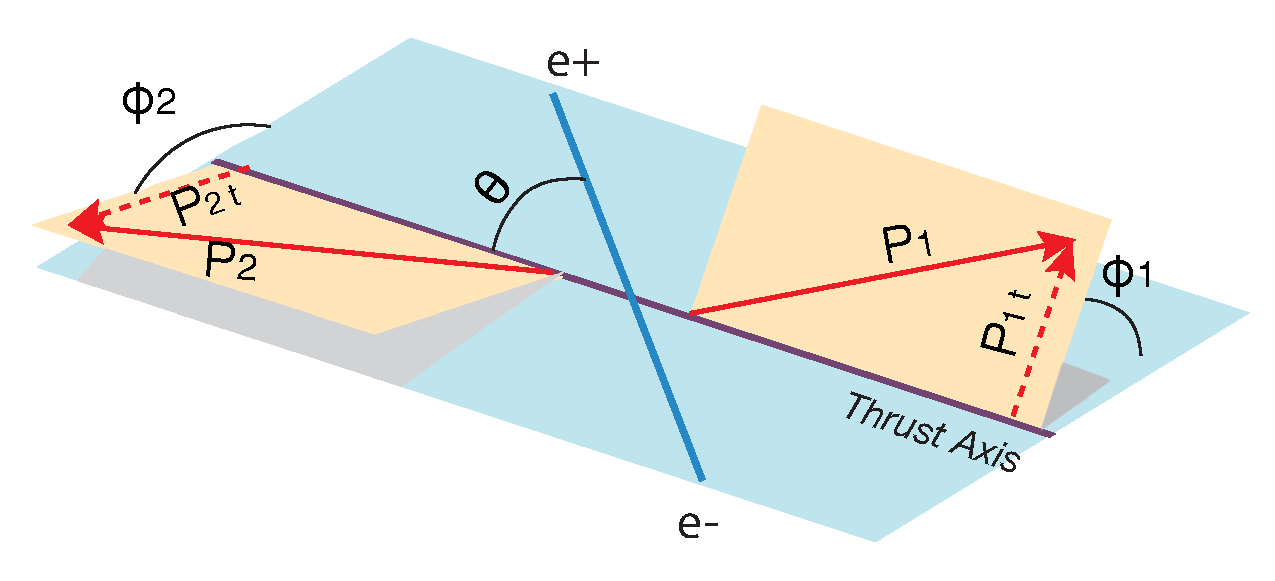
\includegraphics[width=.9\textwidth,natwidth=600,natheight=400]{figure_theory/e+e-_phi1phi2.pdf}
  \caption{Thrust reference frame.}
  \label{fig:phi1phi2frame}
\end{figure}

In this study, the quark-antiquark axis is used as the reference framesto calculate the differential cross subsection~\cite{BoerThesis}. However, the direction of quark-antiquark pair is not detectable and thrust axis can used as an approximation. Fig.~\ref{fig:phi1phi2frame} shows the frame that uses thrust axis as reference. Thrust axis~($\boldsymbol{\hat{n}}$) can be obtained by  maximizing:
\begin{equation}
t=\sum_h\frac{|\boldsymbol{P_h\cdot\hat{n}}|}{|P_h|}.
\end{equation}
Here the summation runs over all stable final state particles. In experiment, not all state particles can be collected thus the reconstructed thrust axis is not accurate. This effect will be discussed and corrected in subsection~\ref{sec:smearingcorrection}. 

In this reference frame, the differential cross subsection is dependent on fractional energy~($z$), Collins angle~($\phi$) and expressed as~\cite{BoerThesis}:
\begin{equation}
\begin{aligned}
\frac{d\sigma(e^+e^-\rightarrow h_1h_2X)}{d\Omega dz_1dz_2 d\phi_1d\phi_2}=\Sigma_{q,\bar{q}} \frac{2\alpha^2}{Q^2}\frac{e_q^2}{4}z^2_1z^2_2\{ (1+\cos^2\theta)D_1^{q,[0]}(z_1)\bar{D}_1^{q,[0]}(z_2) \\
+\sin^2\theta\cos(\phi_1+\phi_2)H_1^{\bot,[1],q}(z_1)\bar{H}_1^{\bot,[1],q}(z_2)\},
\end{aligned}
\label{eqn:cross_subsection_ee}
\end{equation}
where the sum sign adds all quark flavors accessible at the center-of-mass energy~\cite{BoerThesis},  with $\theta$ the angle between the colliding beam and the initial quarks. The charge carried by each quark is written as $e_q$.

Equation.~\ref{eqn:cross_subsection_ee} can be simplified as:
\begin{equation}
d\sigma \sim A+B\cos(\phi_1+\phi_2)H^{\bot q}_{h1}\bar{H}^{\bot q}_{h2}.
\label{eqn:FF2}
\end{equation}
\noindent where in Eq.~\eqref{eqn:FF2}, $A(y)=(\frac{1}{2}-y+y^2)$ and $B(y)=y(1-y)$. In the CMS, $A$ and $B$ can be described as $A(y)=\frac{1}{4}(1+\cos^2\theta)$ and $B(y)=\frac{1}{4}\sin^2\theta$. 

Collins Fragmentation Function appears in the first order transverse moment as~\cite{AsyInPolarizedHadronProductionInEE}:
\begin{equation}
H_1^{\bot(1)}=z^2\int d^2 \boldsymbol{k}_T \frac{\boldsymbol{k}_T^2}{2M^2} H_1^{\bot}(z,z^2\boldsymbol{k}_T^2)
\label{eqn:firstmomet}
\end{equation}
\noindent where $H^{\bot q}_1(z,P^2_{h\bot})$ is the Collins FF. Similarly with subsection~\ref{sec:SIDIScrosssubsection}, $z$ is defined as the fractional energy of the hadron $z\approx -\frac{2P_h\cdot q}{Q^2}=\frac{2*E_h}{\sqrt{S}}$. The last item in Eq.~\eqref{eqn:FF1} is dependent on the quark spin direction and hence the transverse distribution function will lead to an asymmetric azimuthal angle distribution as shown in Eq.~\eqref{eqn:tssa}.   

\subsection{Observable}
\label{sec:observable}
A hadron pair is composed of hadrons from different hemispheres, which means:
\begin{equation}
sign=(P_1 \cdot \hat{n})(P_2\cdot \hat{n}) < 0 .
\end{equation}
If the two hadrons in different hemispheres are measured simultaneously, the Collins asymmetry will be proportional to $\cos(\phi_1+\phi_2)$. The angles $\phi_1$ and $\phi_2$ are shown in Fig.~\ref{fig:phi1phi2frame} and can be calculated using
\begin{equation}
%\phi_i=\frac{\hat{\boldsymbol{n}}}{|\hat{\boldsymbol{n}|}}\cdot(\frac{\hat{\boldsymbol{z}}\times\hat{\boldsymbol{n}}}{|\hat{\boldsymbol{z}}||\hat{\boldsymbol{n}}|}\times\frac{\hat{\boldsymbol{n}}\times\hat{\boldsymbol{P}_{h,i}}}{|\hat{\boldsymbol{n}}||\hat{\boldsymbol{P}_{h,i}}|})\arccos(\frac{\hat{\boldsymbol{z}}\times\hat{\boldsymbol{n}}}{|\hat{\boldsymbol{z}}||\hat{\boldsymbol{n}}|}\times\frac{\hat{\boldsymbol{n}}\times\hat{\boldsymbol{P}_{h,i}}}{|\hat{\boldsymbol{n}}||\hat{\boldsymbol{P}_{h,i}}|}),
\phi_i=sgn[\hat{\boldsymbol{n}}\cdot \{ (\boldsymbol{z}\times\hat{\boldsymbol{n}})\times(\hat{\boldsymbol{n}}\times{\boldsymbol{P}_{h,i}})\}]\times \arccos(\frac{\hat{\boldsymbol{z}}\times\hat{\boldsymbol{n}}}{|\hat{\boldsymbol{z}}\times\hat{\boldsymbol{n}}|}\times\frac{\hat{\boldsymbol{n}}\times{\boldsymbol{P}_{h,i}}}{|\hat{\boldsymbol{n}}\times{\boldsymbol{P}_{h,i}}|}),
\label{eqn:collinsangledefine2}
\end{equation}
here $i$ stands for the hadron from first or second hemisphere and $\boldsymbol{z}$ is the unit vector along the beam direction.

The Collins angle of a hadron pair is $\phi_{12} \equiv \phi_1+\phi_2$. The di-hadron yield $N_{12}=N_{12}(\phi_1+\phi_2)$ divided by the average yield gives the normalized rate $R_{12}=\nicefrac{N_{12}}{\langle  N_{12}\rangle}$. Considering the $\cos(\phi_1+\phi_2)$ modulation, $R_{12}$ can be parameterized as $R_{12}=a_{12}(\theta,z_1,z_2)\cos(\phi_1+\phi_2)+b_{12}$ with the azimuthal asymmetry
\begin{equation}
a_{12}(\theta,z_1,z_2)=\frac{\sin^2\theta}{1+\cos^2\theta}\frac{\sum\limits_{a}e^2_aH^{\bot q}_1(z_1,P^2_{h1\bot})\bar{H}^{\bot q}_1(z_2,P^2_{h2\bot})}{\sum\limits_{a}e^2_aD^q_1(z,P^2_{h\bot})\bar{D}^q_1(z,P^2_{h\bot})}.
\end{equation}

As will be discussed later (see subsection~\ref{sec:dataselection}), the azimuthal distribution can be strongly distorted due to acceptance effects. Furthermore, initial-state radiation (ISR) and gluon radiation introduce cosine modulations similar to the ones arising from the Collins effect. To remedy those effects the double ratio (DR) method, in which we calculate the ratio of normalized distribution between certain different kinds of hadron pairs, can be used as the effects are assumed to be charge independent and thus largely cancel during the ratio calculation~\cite{ChargedPionResult,CollinsInSIDISandEE}. To apply the double ratio method, two hadrons in different hemispheres are combined together as a hadron pair. For each hadron, the Collins angle is calculated using Eq.~\eqref{eqn:collinsangledefine2}. For example, in the charged pion analysis, the double ratio was designed to be the ratio of unlike sign pairs ($\pi^+\pi^-$) to like sign pairs ($\pi^+\pi^+$ and $\pi^-\pi^-$).

%For the Collins effect, the Collins FF can be separated into favored and unfavored parts according to which flavor goes into the hadron where charge-conjugation and isospin symmetry arguments have been used~\cite{CollinsInSIDISandEE}:
Fragmentation functions are often categorized into favored and disfavored ones, depending on whether or not the fragmenting-quark flavor is part of the valence structure of the hadron formed. For charged pions, employing charge-symmetry and isospin asymmetry, FFs are 
\begin{equation}
\begin{aligned}
D^{fav}=D^{u/{\pi^+}}=D^{d/{\pi^-}}=D^{\bar{u}/{\pi^-}}=D^{\bar{d}/{\pi^+}}\\
D^{dis}=D^{u/{\pi^-}}=D^{d/{\pi^+}}=D^{\bar{u}/{\pi^+}}=D^{\bar{d}/{\pi^-}}.
\label{eqn:FF4}
\end{aligned}
\end{equation}
The fragmentation functions of $\pi^0$ consist of both favored and disfavored FFs~\cite{FoundationsofpQCD},
\begin{equation}
\begin{aligned}
D^{u/{\pi^0}}=D^{\bar{u}/{\pi^0}}=D^{d/{\pi^0}}=D^{\bar{d}/{\pi^0}}=D^{dis}+D^{fav}.
\label{eqn:FF4pi0}
\end{aligned}
\end{equation}
Besides light quarks, we also consider the contribution of strange quarks. A common assumption is that the probability for strange-quark fragments into charged pions is the same as the light-quark disfavored ones, as it also requires generating the two valence quarks forming the pion, thus
\begin{equation}
D^{dis}_{s\rightarrow\pi}=D^{s/{\pi^-}}=D^{s/{\pi^+}}=D^{s/{\pi^0}}.
\end{equation}
In this note, double ratios for neutral mesons are designated as:
\begin{equation}
\label{eqn:FF6}
\begin{aligned}
A_{12}^{\pi^0}=\frac{A^{0\pm}_{12}}{A^L_{12}}=\frac{\pi^0\pi^++\pi^0\pi^-}{\pi^+\pi^++\pi^-\pi^-}\\
A_{12}^{\eta}=\frac{A^{\eta\pm}_{12}}{A^L_{12}}=\frac{\eta\pi^++\eta\pi^-}{\pi^+\pi^++\pi^-\pi^-}.
\end{aligned}
\end{equation}
Asymmetries after applying the double ratio, for instance, like sign pairs $A^L_{12}$ and $\pi^0\pi^{\pm}$ pairs $A^{0\pm}_{12}$, can be expressed in favored and unfavored FF~\cite{ChargedPionResult}:

\begin{multline}
A_{12}^{\pi^0}=\frac{A^{0\pm}_{12}}{A^L_{12}}=1+\cos(\phi_1+\phi_2)\frac{\sin^2(\theta)}{1+\cos^2(\theta)} \\
\times\bigg\{\frac{5(H^{\bot,fav}_1+H^{\bot,dis}_1)(H^{\bot,dis}_2+H^{\bot,fav}_2)+2H^{\bot,dis}_{1,s\rightarrow\pi}H^{\bot,dis}_{2,s\rightarrow\pi}}{5(D^{\bot,fav}_1+D^{\bot,dis}_1)(D^{\bot,dis}_2+D^{\bot,fav}_2)+2D^{dis}_{1,s\rightarrow\pi}D^{dis}_{2,s\rightarrow\pi})}\\
-\frac{5H^{\bot,fav}_1H^{\bot,dis}_2+5H^{\bot,dis}_1H^{\bot,fav}_2+2H^{\bot,dis}_{1,s\rightarrow\pi}H^{\bot,dis}_{2,s\rightarrow\pi}}{5D^{\bot,fav}_1D^{\bot,dis}_2+5D^{\bot,dis}_1D^{\bot,fav}_2+2D^{dis}_{1,s\rightarrow\pi}D^{dis}_{2,s\rightarrow\pi}} \bigg\}.
\label{eqn:FF5}
\end{multline}
%Due to the differing valence structure of the $\eta$, the FFs composition the relations above~\ref{eqn:FF5} read differently:

To study the FFs expression of $\eta$, due to the differeing valence structure with $\pi^0$, we need to reconsider the cases with strange-quark fragments into $\eta$. Neglecting symmetry breaking due to strangeness suppression, the strange-quark FFs can be related to the non-strange ones:
\begin{equation}
\begin{aligned}
D^{u/{\eta}}=D^{d/{\eta}}=D^{\bar{u}/{\eta}}=D^{\bar{d}/{\eta}}=D^{s/{\eta}}=D^{\bar{s}/{\eta}}=D^{fav}+D^{dis}.
\label{eqn:FFetaquark}
\end{aligned}
\end{equation}
which results in the following expression for the double ratio:
\begin{multline}
A_{12}^{\eta}=\frac{A^{\eta\pm}_{12}}{A^L_{12}}=1+\cos(\phi_1+\phi_2)\frac{\sin^2(\theta)}{1+\cos^2(\theta)} \\
\times\bigg\{\frac{5(H^{\bot,fav}_1+H^{\bot,dis}_1)(H^{\bot,dis}_2+H^{\bot,fav}_2)+2(H^{\bot,fav}_{1,s\rightarrow\eta}+H^{\bot,dis}_{1,s\rightarrow\eta})H^{\bot,dis}_{2,s\rightarrow\pi}}{5(D^{\bot,fav}_1+D^{\bot,dis}_1)(D^{\bot,dis}_2+D^{\bot,fav}_2)+2(D^{dis}_{1,s\rightarrow\eta}+D^{dis}_{1,s\rightarrow\eta})D^{dis}_{2,s\rightarrow\pi})}\\
-\frac{5H^{\bot,fav}_1H^{\bot,dis}_2+5H^{\bot,dis}_1H^{\bot,fav}_2+2H^{\bot,dis}_{1,s\rightarrow\pi}H^{\bot,dis}_{2,s\rightarrow\pi}}{5D^{\bot,fav}_1D^{\bot,dis}_2+5D^{\bot,dis}_1D^{\bot,fav}_2+2D^{dis}_{1,s\rightarrow\pi}D^{dis}_{2,s\rightarrow\pi}} \bigg\}.
\label{eqn:FF5eta}
\end{multline}

The the parameterization $A_{12}*\cos(\phi_1+\phi_2)$ is fitted to the final double ratio distribution, where the amplitude $A_{12}$ is the azimuthal asymmetry that is measured in this note. 